% 2
%\chapter{準備}
\section{準備}

% 2.1
\subsection{基本的用語}
集合$A$の$k$個の要素からなる部分集合の族を$[A]^k$で表す.グラフとは,$E\subseteq [V]^2$を満たす集合の組$G=(V,E)$のことである.$V$の要素をグラフ$G$の頂点と,$E$の要素を$G$の辺と呼ぶ.頂点$v$と辺$e$に対して,$v\in e$となるとき,$v$は$e$に接続するといい,$e$を$v$の接続辺と呼ぶ.1つの辺に接続する2つの頂点はその辺の端点と呼ぶ.頂点$v$の接続辺で$E$に属すもの全体の集合を$E(v)$で表す.グラフ$G$に辺$\{x,y\}$があるとき,$G$の2つの頂点$x,y$は隣接するといい,互いに他方の隣接点と呼ぶ.$G=(V,E)$と$G'=(V',E')$を2つのグラフとする.その頂点集合の間の全単射$\phi :V\rightarrow V'$で,全ての$x,y\in V$に対して$\{x,y\}\in E\Leftrightarrow \{\phi(x),\phi(y)\}\in E'$を満たすとき$G$と$G'$は同型であるという.$G\cup G'= (V\cup V',E\cup E'),G\cap G'= (V\cap V',E\cap E')$とおく.$G\cap G'=\emptyset$のとき$G$と$G'$は交わらない.$V'\subseteq V$かつ$E'\subseteq E$ならば,$G'$を$G$の部分グラフと呼ぶ.$G'\subseteq G$であり,$G'$が$x,y\in V'$となる辺$\{x,y\}\in E$をすべて含むとき,$G'$は$G$の誘導部分グラフであるという.頂点$v$の次数$d_G(v)$とは,$v$の接続辺の個数$|E(v)|$である.$G$が明らかなときは,$d_G(v)$を単に$d(v)$と記す.次数の最大値$\Delta (G)= \max \{d(v)\mid v\in V\}$を最大次数という.道とは次のように与えられる空でないグラフ$P=(V,E)$のことである.
\begin{align*}
  V & = \{x_0,x_1,\ldots,x_k\},\\
  E & = \{\{x_0,x_1\},\{x_1,x_2\},\ldots,\{x_{k-1},x_k\}\}\\
    & (x_i\neq x_j,0\leq i<j\leq k)
\end{align*}
$U$を任意の頂点(または辺)の集合とするとき,$G+U$は,$G$に$U$に属す頂点とその接続辺をすべて追加して得られるグラフである.$P$が道で,$k\geq 3$のとき,グラフ$C=P+\{\{x_{k-1},x_0\}\}$を閉路と呼ぶ.グラフ$G$に対して,その頂点集合を$V(G)$,辺集合を$E(G)$と記す.頂点の集合$A,B$に対して,$V(P)\cap A=\{x_0\}$かつ$V(P)\cap B=\{x_k\}$となるとき,$P=(x_0\ldots x_k)$を$A$-$B$道と呼ぶ.$A=\{x\},B=\{y\}$のとき,$A$-$B$道を単に$x$-$y$道と呼ぶ.2つの頂点$x,y$の距離$d_G(x,y)$とは,$G$における最短の$x$-$y$道の長さである.

% 2.2
\subsection{木}
グラフ理論において,木とはすべての頂点が連結しており,閉路(サイクル)を持たないグラフを指す.特に,根と呼ばれる頂点を1つ指定した木のことを\textbf{根付き木(rooted tree)}と呼ぶ.特別な注釈がない限り,本論文では木という用語は根付き木を意味するものとし,以降は根付き木を単に木と記述する.

$\Sigma$および$\Lambda$を有限アルファベット,$X$を無限アルファベットとする.ただし,$(\Sigma\cup\Lambda)\cap X=\emptyset$が成り立つものとする.また,頂点集合$V_T$と辺集合$E_T$を持つ木を$T = (V_T, E_T)$とする.$\{u,v\}\in E_T$に対して$u$が$v$より根に近いとき,辺$\{u,v\}$を順序対$(u,v)$で表す.以降,本論文では$(u,v)\in E_T$を$\{u,v\}\in E_T$かつ$u$が$v$より根に近いという意味で用いる.さらに,$(u,v)\in E_T$のとき,頂点$u$を$v$の親,$v$を$u$の子と呼ぶ.また,根ではない次数が1の頂点を葉と呼び,葉に接続する辺または変数を\textbf{葉辺(leaf edge)}と呼ぶ.木の頂点集合$V_T$の各頂点には$\Sigma$に属す記号が,辺集合$E_T$の各辺には$\Lambda$に属す記号がそれぞれラベル付けされているものとする.$\Sigma$に属す記号を頂点ラベル,$\Lambda$に属す記号を辺ラベルと呼ぶ.また,$X$に属す記号を変数ラベルと呼び,各$x \in X$にはランクと呼ばれる1以上の整数が割り当てられていると仮定する.

% 図2.1
\begin{figure}[tb]
  \centering
  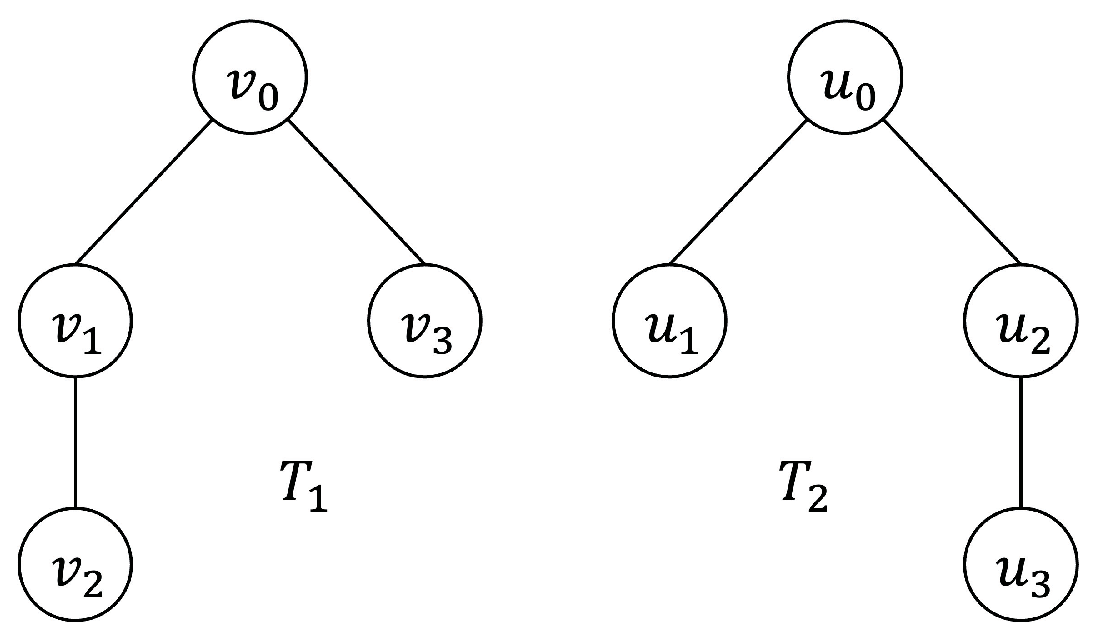
\includegraphics[scale=0.28]{fig/fig-sibling_relationship.eps}
  \caption{$T_1$と$T_2$は,無順序木のときは同型,順序木のときは同型ではない.}\label{fig:sibling_relationship}
\end{figure}

